%%%%%%%%%%%%%%%%%%%%%%%%%% author.tex %%%%%%%%%%%%%%%%%%%%%%%%%
%
% sample root file for your contribution to a "contributed book"
%
% "contributed book"
%
% Use this file as a template for your own input.
%
%%%%%%%%%%%%%%%%%%%%%%%% Springer-Verlag %%%%%%%%%%%%%%%%%%%%%%%%%%


% RECOMMENDED %%%%%%%%%%%%%%%%%%%%%%%%%%%%%%%%%%%%%%%%%%%%%%%%%%%
\documentclass{svmult}

% choose options for [] as required from the list
% in the Reference Guide, Sect. 2.2

\usepackage{makeidx}         % allows index generation
\usepackage{graphicx}        % standard LaTeX graphics tool
                             % when including figure files
\usepackage{multicol}        % used for the two-column index
\usepackage[bottom]{footmisc}% places footnotes at page bottom
% etc.
% see the list of further useful packages
% in the Reference Guide, Sects. 2.3, 3.1-3.3

\makeindex             % used for the subject index
                       % please use the style sprmidx.sty with
                       % your makeindex program


%%%%%%%%%%%%%%%%%%%%%%%%%%%%%%%%%%%%%%%%%%%%%%%%%%%%%%%%%%%%%%%%%%%%%

\usepackage{algorithm}
\usepackage{algpseudocode}
\usepackage{amssymb}
\usepackage{amsmath}
\usepackage{url}
\begin{document}

\title*{Automated Edge Grid Generation Based on Arc Length Optimization}
% Use \titlerunning{Short Title} for an abbreviated version of
% your contribution title if the original one is too long
\author{David McLaurin\inst{1}\and
Suzanne M. Shontz\inst{2}}
% Use \authorrunning{Short Title} for an abbreviated version of
% your contribution title if the original one is too long
\institute{High Performance Computing Collaboratory,
           Center for Advance Vehicular Systems,
	       Graduate Program in Computational Engineering,
		   Mississippi State University, Mississippi State, MS
		   \texttt{d.mclaurin@msstate.edu}
\and Department of Mathematics and Statistics,
     Department of Computer Science and Engineering,
	 Center for Computational Sciences,
	 Graduate Program in Computational Engineering,
	 Mississippi State University, Mississippi State, MS
     \texttt{sshontz@math.msstate.edu} }
%
% Use the package "url.sty" to avoid
% problems with special characters
% used in your e-mail or web address
%
\maketitle

%% main text
\begin{abstract}
Computational design and analysis has become a fundamental part of industry and academia for use in research, development, and manufacturing.  In general, the accuracy of a computational analysis depends heavily on the fidelity of the computational representation of a real-world object or phenomenon. Most mesh generation strategies focus on element quality--with the justification being that downstream applications require high quality geometries in order to achieve a desired level of accuracy. However, element quality should be secondary to accurately representing the underly physical object or phenomenon. This work seeks to improve the process of creating a computational model of an object of interest by accelerating the process of mesh generation by reducing the need for (often) manual intervention. This acceleration will be accomplished by automatically generating \textit{optimal} discretizations of curves by minimizing the \textit{arc-length deficit}. Methods were developed to generate optimal discretizations through local or global optimization. Results are presented showing the robustness and accuracy of the developed methods along with a discussion as to how to implement the developed methods into an existing mesh generator.
\end{abstract}

% Introduction Document
\section{Introduction}Computational design and analysis has become a fundamental part of industry and academia for use in research, development, and manufacturing. In general, the accuracy of a computational analysis depends heavily on the fidelity of the computational representation of a real-world object or phenomenon. However, the task of creating high fidelity models of an actual geometry can be time-consuming--sometimes consuming up to seventy-five percent of the time required to produce a solution \cite{bischoff05}. This work seeks to improve the process of creating a computational model of an object of interest by accelerating the process of mesh generation. Below in Figure-\ref{GridGenerationProcess} an example of a mesh generation hierarchy can be seen. In general, a valid volume grid (three-dimensional) is bounded by surface grids (two-dimensional); and surface grids are bounded by edge-grids (one-dimensional). At the start of the grid generation hierarchy are point spacing values at the end points of analytical or parametric curves—which bound the edge-grids. In most cases, volume-grid generation is a highly automated procedure—once the bounding surfaces are generated. The same generalization can be made for surface-grids and edge-grids. Algorithms that use automated point creation/insertion for mesh generation of one-, two-, and three-dimensional geometries are ubiquitous [REFERENCES, CUBIT, Delaunay, AFLR]. However the authors are only aware of one such automated scheme for setting point spacing values for more automated mesh generation \cite{mclaurin12}.\\

\begin{figure}[h!]
 \center{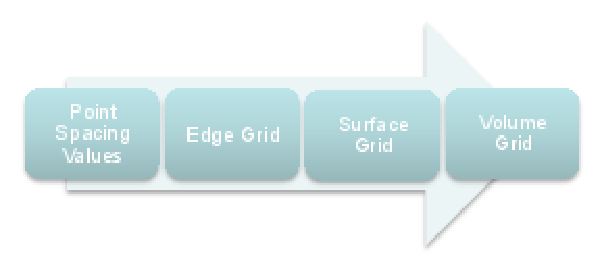
\includegraphics[width=0.8\textwidth]
  {Figures/GridGenProcess.eps}}
 \caption{\label{GridGenerationProcess} Specified point spacings and final point distribution for a surface edge \cite{thompson98}}
\end{figure}

The computation involved with edge-grid generation is trivial when compared to volume-grid generation—even with high-order NURBS curves. However, the point spacing values at the end points of curves have to be set manually in order to satisfy a desired length scale. This manual process is time consuming. If geometry repair (gluing, trimming, etc…) is not considered, the amount of user input required to generate a volume grid can be concentrated on the lowest levels of the grid generation hierarchy. In addition, if the edge-grids are not generated appropriately then the errors present there, such as overly dense or sparse spacing, will be propagated up the hierarchy and be present in each subsequent higher-dimensional entity. In order to accelerate the process of generating edge grids, some degree of automation is needed to help deal with common issues associated with undesirable edge-grids.

The proposed algorithm is a general-use method that can be applied to any ``digital curve'' regardless of its representation. This is due to every step being developed without the use of derivatives. Most other methods operate on a specific type of curve, such as NURBS or B-splines, and use the specific information available for the type of curve in use. While in the field of CAD NURBS curves are the de-facto standard, in other fields, such as pattern-recognition, other types of digital curves, such as parametric, are more common[REFERENCES]. T-splines are also becoming more popular in applications such as isogeometric analysis [REFERENCES, Thomas Hughes]. Therefore a general algorithm that does not require derivative information to generate a suitable edge grid was developed. A result of not using derivatives is that each step in the algorithm is robust to large changes in derivatives or curves that are not ``well behaved''---highly oscillatory for instance.

The justification for the development of these methods lies in the need for an automated way of setting point spacing values on curves. This process can only be automated if some way of judging ``how well'' an edge grid represents a curve is present. To this end, two related methods of generating edge grids through constrained optimization are detailed below. Further discussion of element quality, robustness, and a framework for implementing the information associated with an optimal edge grid into an existing grid generator is also presented. Generating edge grids in a more automated fashion accelerates the process of surface grid generation---and ultimately volume grid generation. Using the detailed methods, or any other automated method for setting point spacings does not change the number of steps required for grid generation. However, it does reduce the number of manual steps involved in starting the process.



%Related Work/ Background/ Lit Review
\section{Related Work}
In general, grid generation is a name for any process that creates a grid.  
For example, the advancing-front algorithm advances boundaries into space 
to generate a grid \cite{lohner88}.  Other methods generate grids from 
iterative refinement or enrichment from initial, coarse 
configurations[cite].  Usually the benchmark for separating the two 
methods, generation and refinement, are the prioritization of grid quality 
and grid accuracy (both of these issues will be addressed later).  From a 
standard text \cite{thompson98}: One dimensional grids, or edge grids, 
\begin{quotation} \noindent ``...are created using a one-dimensional 
version of the standard grid generation procedure.  This ensures that 
point distribution and growth rates are fully compatible for optimal final 
grid quality.  For each edge or segment the point spacing is specified at 
both ends... Edge grid generation is then used to produce the point 
distribution...'' \end{quotation} An example of this can be seen below in Figure-\ref{EdgeGrid_HandbookOfGridGeneration} where the point spacing distributions are df1 and df2.

\begin{figure}[h!]
  \center{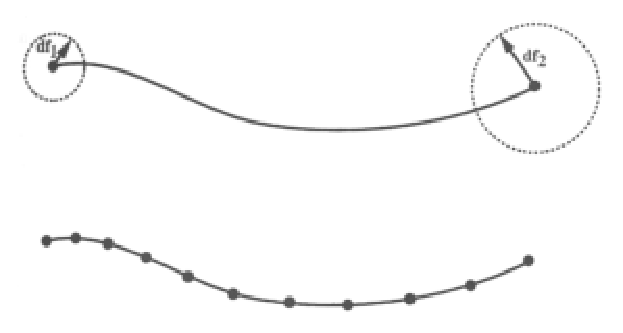
\includegraphics[width=0.8\textwidth]
    {Figures/EdgeGrid_HandbookOfGridGeneration.eps}}
  \caption{\label{EdgeGrid_HandbookOfGridGeneration} Caption}
\end{figure}

\noindent In the example above, the edge grid generation process produces good quality grids from the combination of geometric growth rates and smoothing.  However, the process requires input: point spacing values.  If the point spacing values are not appropriate then the geometry can be under and/or over sampled for the intended use.  That fact is not an indictment of the grid generation process, but instead implies that the final grid is heavily dependent on the inputs.  In addition, if some way of controlling the point spacing in the middle of a curve is not present, then more points could be wasted/omitted in an attempt to accurately represent geometry.

Instead of setting appropriate point spacing values and using common grid generation techniques, other efforts have gone into creating a locally or globally ``optimal'' edge grid.  Many names have been assigned to this particular task, but the underlying goal is very similar—represent a curve as accurately as possible—whatever that means for each application.  For example, \cite{laug04} first linearized the interface between curves in order to simplify the process of generating edge grids and surface grids on topologically adjacent patches.  Other ``geometry aware'' or ``curvature based'' approaches have been developed.  One such application is for discretizing curves for use in level set methods \cite{macklin06}.  Others include energy minimization \cite{hofer04}, curvature minimization \cite{zehiry10}, and angle minimization \cite{ebeida10}.



%Discretization Error
\section{Discretization Error}
The accuracy, or discretization error, of a piecewise, linear 
representation ($discretization$) of an analytical curve ($curve$) in 
$R^3$ can be defined in many ways depending on the intended application.  
The error associated with the $discretization$ is discussed in terms of 
the ``deviation'' from the $curve$—most often quantified by calculating or 
approximating the distance from the $curve$ for each linear segment in the 
$discretization$, or the area of the ruled surface between a curve-piece 
and the segment representing that part of the $curve$.  Another way of 
quantifying the error associated with a $discretization$ would be to 
consider how well it approximates the arc length of the $curve$ it 
represents.  In general the arc length is not known a priori, but 
depending on the underlying representation it can be calculated exactly 
(parametric or analytical) or can be estimated (Bezier).  One of the goals 
of this method was to be ``general'' in that it should be independent of 
the underlying geometric representation.  Therefore a method that requires the 
arc-length of the underlying geometry violates the aforementioned concept 
of ``generality'' and restricts the applications for which the proposed 
method could be applied.  Some other way of determining/generating an edge 
grid based on arc length is needed.  This process will be detailed later.

Arc-length convergence of a $discretization$ is a sufficient condition for 
other schemes of edge grid generation/refinement.  That is: if the 
difference between the arc length of the $curve$ and the sum of the 
segments in the $discretization$ approaches zero then that is sufficient 
to conclude that the distance between the $discretization$ and the $curve$ 
is also approaching zero, also the angles between segments approaches 180 
degrees.  However, the converse of that statement is not true.  The 
pathological case of a highly oscillatory, low amplitude $curve$ 
approximated by two straight lines shows that a $discretization$ of a 
$curve$ can have a small ``deviation'' or angles between segments but be a 
poor estimate for arc length.  Another pathological case is a 
``non-convex'' $curve$ where the parameterization goes well ``outside'' of 
the segment.



% Discrete Curvature Approximation
\section{Discrete Curvature Approximation}
The concept of ``deviation'' as defined above is relatively straightforward and intuitive. However, another related way of describing ``how well'' a \textit{discretization} represents a \textit{curve} is the degree to which the discrete representation approximates curvature -- where curvature is defined as the amount of ``bend'' in a \textit{curve} or surface, or ``how much'' a \textit{curve} or surface ``differs'' from a straight line or plane (words in quotes are subject to gradation). First, however, curvature must be defined in such a way that a discrete approximation is meaningful and appropriate. In relevant literature there are many ways to estimate curvature \cite{hermann07}. Some of it bears repeating because it is germane to what is being discussed here: Consider the following planar \textit{curve}, C, at point P. At a given point P there exists an osculating circle, O, of radius r such that the circle has the same tangent as the \textit{curve} C as well as the same radius of curvature \cite{gray97}. \\

\begin{figure}[h!]
  \center{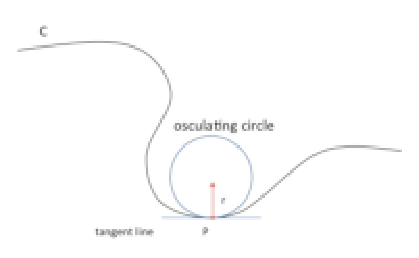
\includegraphics
    {Figures/OsculatingCircle.eps}}
  \caption{\label{OsculatingCircle} Osculating Circle of a Planar Curve}
\end{figure}

\noindent Just as the tangent line is the line best approximating a \textit{curve} at a point, the osculating circle is the best circle that approximates the \textit{curve} a point. Ignoring degenerate \textit{curve}s such as straight lines, the osculating circle of a given \textit{curve} at a given point is unique \cite{gray97}. The radius, r, of the osculating circle at a given point on a \textit{curve} is equal to the radius of curvature, R, which is the reciprocal of curvature, $\kappa$--sometimes called the ``first curvature'' \cite{kreyszig91}. For a two-dimensional \textit{curve} of the form $y=f(x)$, the equation for curvature is:
\[ 
R=\frac{1}{\kappa} \textnormal{, where } 
\kappa=\frac{\frac{d^2y}{dx^2}}{[1+\frac{dy}{dx}^2 ]^\frac{3}{2}}. 
\]
\noindent This quantity, $\kappa$, necessarily includes the calculation of 
derivatives which, depending on the representation of the underlying geometrical description, could be relatively costly. Therefore, this is avoided by defining this radius of curvature on a segment or at a point in the \textit{discretization} without the use of derivatives. This is discussed in the following paragraphs.

A value of curvature can be calculated for each edge in the \textit{discretization} by considering the corresponding osculating circle on a given edge. The osculating circle here (circle, Figure 2) can be approximated by considering the circumscribed circle (circumcircle) \cite{casey1888} defined by the two end points of the edge, P0 and P1, and a point, P, between them in the \textit{curve} parameterization—the radius of the circumcircle will be referred to as the discrete radius of curvature.

\begin{figure}[h!]
  \center{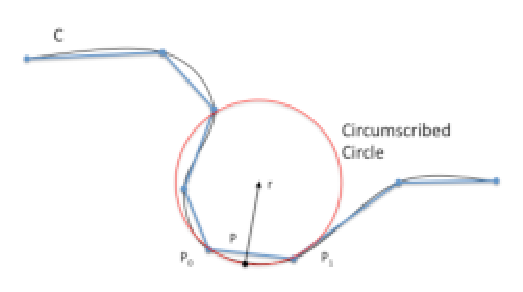
\includegraphics
    {Figures/CircumscribedCircle.eps}}
  \caption{\label{CircumscribedCircle} Caption}
\end{figure}


The method of choosing this point, P, and its importance to an accurate mesh refinement will be detailed later. This definition/approximation of the radius of curvature of the \textit{curve}/\textit{discretization} is useful for this application, but exhibits scale-dependence. The discrete radius of curvature alone is not sufficient to determine how well a segment approximates the curvature. The discrete radius of curvature must be given some context. In other words: it must be compared to the local feature size in order to determine if the segment is an accurate representation. Another problem with comparing the radius of curvature and the discrete radius of curvature is that as the \textit{discretization} becomes more refined the discrete radius of curvature approaches infinity and therefore diverges from the analytical value at that point. Stated another way, as the sum of the length of the segments in the \textit{discretization} converges to the actual length of the \textit{curve}, the discrete radius of curvature of each segment approaches infinity. Therefore, a quantity is needed that is scale-independent that converges to a computer-representable value as the \textit{discretization} becomes more refined.

Consider a circular segment, which represents the \textit{curve}, $s$.  
The corresponding chord, which represents a segment in the 
\textit{discretization}, $a$, and saggitta--which represents the 
``deviation'' of the segment away from the \textit{curve}, $h$, is shown 
in Figure~\ref{CircleGeometry}.

\begin{figure}
  \center{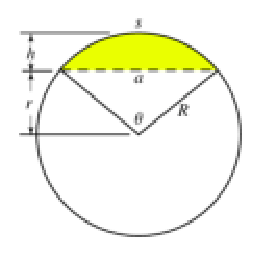
\includegraphics
    {Figures/CircleGeometry.eps}}
  \caption{\label{CircleGeometry} Caption}
\end{figure}.

\begin{theorem}
As the length of $a$ approaches the length of $s$, the length of $h$ goes 
to zero, therefore the radius of the circle, $R$, goes to infinity.  
\end{theorem}

\begin{proof}
First, 
\begin{eqnarray}
\begin{array}{lcl}
a & = & \sqrt{R^2+r^2}=2*\sqrt{(h*(2*R-h)}.
\end{array}
\end{eqnarray}
Upon rearranging, we obtain
\begin{eqnarray}
\begin{array}{lcl}
R & = & \frac{(\frac{a}{2})^2*\frac{1}{h}+h}{2}=
\frac{a^2+4*h^2}{8*h}=\frac{a^2}{8*h}+\frac{h}{2}.
\end{array}
\end{eqnarray}
Finally,
\begin{eqnarray}
\begin{array}{lcl}
\lim_{h\to0} (\frac{a^2}{(8*h)}+\frac{h}{2}) & = & \infty.
\end{array}
\end{eqnarray}
\end{proof}

Given the aforementioned proof, if the discrete curvature radius is 
divided by the length of the corresponding segment on the \textit{curve}, then it’s value approaches zero. This is a scale independent measure that converges to a computer representable number as the \textit{discretization} approaches the length of the \textit{curve}. The parameter is known as the curvature ratio. It is an intuitive measure that relates ``how far'' the \textit{curve} deviates from the segment that is representing it as the ratio of those lengths. Consider a point on a \textit{curve} between two endpoints of a segment of a \textit{discretization}, as seen in Figure~\ref{CurvatureRatio}. The length of the segment, $L_i$, is the distance from $P_0$ to $P_1$. The perpendicular distance between the point on the \textit{curve} between the end points and the segment is $L_c$. The three points define a curvature ratio through the ratio of $L_c$ to $L_i$.

\begin{figure}[h!]
  \center{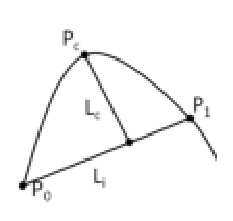
\includegraphics
    {Figures/CurvatureRatio.eps}}
  \caption{\label{CurvatureRatio} $curvature \ ratio=  \frac{L_c}{L_i}$ 
\cite{mclaurin10}}
\end{figure}

\noindent As shown in \cite{mclaurin12}, deviation-based methods are 
intuitive and straightforward to implement. However, drawbacks include the fundamental lack of consistently being able to indicate discretization accuracy for curves that are not ``well-behaved'' between discrete segments.


\section{Refinement via Maximum Curvature Ratio/Deviation}
{\bf{DAVE:  Cite this statement.  I commented out the text.  Consider
adding to another section if appropriate.}}

%One could, for instance, find the maximum value for curvature ratio on 
%the segment to determine whether or not to further subdivide the segment.  
%This is an example of ``deviation-based'' refinement.  For a given segment, 
%the maximum curvature ratio is found where the perpendicular distance 
%between the segment and the curve is maximum.  This might not correspond 
%to the point where the combined arc length of the two new segments is 
%maximally different from the current configuration.  For instance 
%consider the triangle, (\textit{A}, \textit{B}, \textit{C}) with sides of 
%length following the Pythagorean triple (5,12,13) and therefore perimeter 
%of 30.

%\begin{figure}[h!]
%  \center{\includegraphics
%    {Figures/CurvatureRatioTriangles.eps}}
%  \caption{\label{CurvatureRatioTriangles} Caption}
%\end{figure}

%\noindent Additionally consider the triangle (\textit{A}, \textit{B}, 
%\textit{D}) formed with the same base (12) and height (5) as the other 
%triangle.  The perimeter of this triangle, (\textit{A}, \textit{B}, 
%\textit{D}) is 27.62. Using point \textit{C} to increases the length of 
%the segment locally by 150\%, while using point \textit{D} increases the 
%length of the segment by 130.1\%.  Both of these triangles have the same 
%curvature ratio since their bases and heights are identical.  However, as 
%shown the perimeter can vary a not-insignificant amount without changing 
%the curvature ratio of a segment.  Therefore, the curvature ratio is not 
%sufficient to determine whether or not the arc length of the 
%discretization is approaching that of the curve—only that the distance 
%between the discretization and the curve is approaching some value 
%locally.  Using only the curvature ratio, the choice between point 
%\textit{C} and \textit{D} in Figure-\ref{CurvatureRatioTriangles} are 
%equal.  The potential error would get worse if the point \textit{C} were 
%moved further left--demonstrating that the curvature ratio is not always 
%a good indicator of discretization accuracy for curves that aren’t 
%``well-behaved'' between discrete segments.



% Refinement via Arc-Length Deficit
\section{Refinement via Arc-Length Deficit}
Mentioned above, a way of determining ``how well'' a discretization 
approximates a curve is to consider the difference between arc lengths. 
This is another way to determine ``how well'' a $discretization$ captures curvature. Locally, it is important for each segment in the discretization to represent the local geometry present in the curve. If a segment is to be subdivided in order to improve the discretization, then it should be subdivided 
effectively/efficient locally.
%in a way that is most effective/efficient locally. 
Also, if the purpose of the refinement process is to minimize the actual 
arc length minus the discrete arc length, then an optimization problem can 
be formed where an objective function is minimized as the combined length of the segments in the discretization approaches that of the curve.

Let $C(u)$ be a parameterized curve, and $D$ be a discretization of the 
curve comprised of $n_t$ points, $P_i : i \in \{1,...,n_t\}$, and 
segments, $S_j : j \in \{1,...,(n_t-1)\}$. Segment $S_j$ is defined by two successive parametrization values, $u_j$ and $u_{j+1}$. If $L(S)$ is a function that calculates the length of a segment in $(x,y)$ space then the optimization problem can be stated as:
\begin{eqnarray*}
\begin{array}{rcl}
\underset{u_i}{\text{minimize}} \ O & = & -\sum{_{j=1}^{n_t-1}L_j} \\
\text{subject to} \ u_1 & = & a \\
u_1 & < & u_2, \\ 
u_2 & < & u_3, \\
& \vdots & \\
u_{n_t-1} & < & u_{n_t},\\ 
u_{n_t} & = & b.
\end{array}
\end{eqnarray*}

The resulting optimization problem is a mixed integer linear programming 
problem if both the parameterization values and number of interior points 
on the curve are unknown.  Mixed integer linear programming problems can 
be solved by a variety of standard techniques (e.g., \cite{minto}, 
\cite{mosek}, or \cite{symphony}).  However, such problems 
are, in general, NP-hard.  
%Alternatively, the optimization problem would 
%need to be solved several times with an increasing number of interior 
%points until the combined length of the segments in the discretization 
%converged to within a desirable tolerance.  This is also a 
%computationally-expensive solution.  
Although the analysis and computation are straightforward for a fixed 
number of interior points, one would need to specify {\it{a priori}} this 
number, which is impractical.

Instead, in order to derive a practical algorithm that controls the 
number of interior points in the discretization, we add user-defined 
bounds on the distance between points in the discretization.  This turns 
the optimization problem into a linear programming problem.  To this end, 
let $e$ and $m$ represent user-defined lower and upper bounds on the 
distance between points in the discretization, 
respectively.  
%In addition, let $\hat{S}_i$ denote the $i^{th}$ segment 
%in non-parametrized space, i.e., $\hat{S}_i = P_{i+1}-P_i$.  
The bounds 
are easily worked into the set of constraints, where $P_i$ represents a 
point in non-parametrized, $(x,y)$-space as follows: 
\begin{eqnarray*} 
\begin{array}{rcl} 
P_1 & = & \alpha,\\ 
e \leq & L_1 & \leq m \\ 
e \leq & L_2 & \leq m \\ 
e \leq & \vdots & \leq m \\ 
e \leq & L_{n_t-1} & \leq m \\ 
P_{n_t} & = & \beta. 
\end{array} 
\end{eqnarray*}

The definition of lower and upper bounds for the distance between points 
implicitly defines an upper and lower bound for the number of interior 
points. The implicit definition would be in the form of an 
over-constrained problem where solutions did not exist for too many or too 
few points. For instance, too many points could not satisfy the 
minimum-distance set of constraints, and too few points could not satisfy 
the maximum-distance set of constraints. However, explicitly determining 
these bounds for $n_t$ would prove difficult. For example, it could 
involve repeatedly sampling the curve to determine the maximum number of 
e-length segments and the minimum number of m-length segments. This would 
be possible but is inefficient. Another option is to estimate the number 
of points needed \cite{cuilliere97}. However, if $n_t$ is to be estimated, 
then the discretization is not guaranteed to be globally optimal. Therefore, 
a global optimization problem, while possible, is not 
very practical in this case. One of the aims of this work is to 
accelerate the generation of suitable grids for simulation; moving the 
bottleneck for grid generation to the lowest level in the grid generation 
hierarchy just increases the amount of time required to generate a grid. 
The above method does, however, represent a solution to the problem of 
generating automated, optimal edge grids.

Others have attempted dynamic programming methods for generating 
``optimal'' discretizations for digital curves \cite{horng02}. However, in 
general this should prove no more effective than any of the approaches 
mentioned above. It is true that the problem of generating a discretization to accurately represent a curve exhibits optimal substructure, which is defined where ``...an optimal solution can be constructed efficiently from optimal solutions to its subproblems'' \cite{cormen01}. However, the number of distinct subproblems available that represent an optimal solution at a defined error bound can be infinite. Therefore, instead of trying to find an optimal number of nodes required for an optimal discretization (which seems very inefficient), the proposed algorithm will use a divide-and-conquer (recursive) approach to generating an ideal discretization relative to a given tolerance. The combination of the optimized segments represents an optimal discretization for the entire curve.

This would generate an optimal solution using two segments to represent the entire curve -- which can be stated another way as maximizing the perimeter of the triangle formed by the existing segment and the two new segments. The above optimization problem could then be applied recursively to each new segment with $n_t=3$. This process breaks the task of optimizing a discretization for an entire curve into optimizing a simple discretization for smaller section of the curve with the following algorithm. The optimization algorithm described above with $n_t=3$ for a given segment is:

\begin{algorithm}
\caption{Optimization Algorithm with $n_t=3$}\label{alg:localoptimize}
\begin{algorithmic}[1]
\State $n_t = 3$
\State $u_i : i \in \{1,2,3\}$
\State $u_1 $ and $u_3$ define the segment $S_{1,3}$
\Procedure{Local Optimization}{$S_{1,3}$}
  \State $L(S_{1,3}) =\textnormal{ length of segment}$
  \State Place interior point $u_2$ to maximize $L(S_{1,2})+L(S_{2,3})$ within $tolerance$
\EndProcedure
\end{algorithmic}
\end{algorithm}

The above algorithm would be applied for each segment in the 
discretization by:
  
\begin{algorithm}[H]
\caption{Optimization Algorithm for Discretization}\label{alg:discreteoptimize}
\begin{algorithmic}
  \State $D(S_j) : j \in {1}$
  \State push $S_1$ into $list$ \Comment{$list$ is $queue$ if breadth-first, $stack$ if depth-first}
  \While{$list$ is not empty}
    \State pop $S_j$ from $list$
    \If {$S_i$ is optimal}
      \State do nothing
    \Else
      \State optimize $S_j$ with \Cref{alg:localoptimize}
      \State push $S_{i,i+\frac{1}{2}}$ into $list$
      \State push $S_{i+\frac{1}{2},i+1}$ into $list$
    \EndIf
  \EndWhile
\end{algorithmic}
\end{algorithm}

The above algorithm is straightforward and is often referred to as 
adaptive refinement or enrichment (see above). Also, since the 
discretization of the curve exhibits optimal substructure, the starting 
point to the optimization algorithm and the method of refinement or 
enrichment are irrelevant to the extent to which they prevent an optimal 
solution from being generated. However, they obviously contribute 
to the efficiency of the algorithm.

Now to define the optimization part of the above algorithm: Divide and 
conquer can be considered to be based on multi-branched recursion. The 
objects to be constructed at the end of the recursion are the smallest set 
of segments that approximates the arc length of the curve to a defined 
precision. This is not quantifiable without {\it{a priori}} knowledge 
of the arc length of the curve. As discussed above, calculating the length 
of a curve for this application is impractical. So how can the 
``goodness'' of a discretization be measured?  At each step, the 
discretization will be refined on each segment by locally optimizing an 
objective function analogous to the one developed above. In order to 
minimize each segment's objective function, arc-length deficit ($ALD$), 
then a point $P$ has to be placed on the curve on the segment such 
that the new sum of the arc lengths is changed maximally. Since this 
entire project is to be done without calculating derivatives (see reasons 
above), the optimization scheme chosen here is not given access to 
derivative information either. Since the objective function is a 
non-negative planar curve, $(O: C \rightarrow ALD)$, any line search 
method of optimization could be used. However, the method cannot have any 
requirements on differentiability due to the possibility that the 
derivative of $O$ could be discontinuous.

The golden section search method is implemented here, since, unlike the 
bisection method, it meets all of the above criteria and has the 
possibility to converge superlinearly \cite{brent73}.  Alternatively, a 
pattern search~\cite{hopspack}, simplex~\cite{dantzig1,dantzig2}, or 
interior point~\cite{karmarkar} method could be used.  If 
the length of each segment 
locally approaches the portion of the curve it represents (i.e., the 
local objective function is 
minimized), then the global length of the discretization approaches the 
global length of the curve (a restatement of the property of optimal 
substructure). Also, since the optimization algorithm for each segment is 
only concerned about the portion of the curve it represents, then this 
method exhibits scale-independence, which was one of our requirements.

Recursive algorithms require stopping criteria. In this case the stopping 
criteria should not permit the method to infinitely subdivide the curve. 
For instance, the aforementioned minimum and maximum segment lengths can 
be used (and were implemented here). Even though using a minimum edge 
length would prevent the infinite subdivision of the curve, another 
criteria is needed such that the minimum segment length is not needed to 
satisfy the criteria. This stopping criterion could be in the form of a 
delta-segment length. That is, if the new segments' combined length is 
below a defined fraction larger than the existing segment then it should 
not be subdivided. This is a ``pure-greedy'' method of subdivision, in 
that it does not consider the rest of the ``solution'' when deciding to 
stop. One problem with this set of stopping criterion is immediately 
apparent: the ``large'' segments could potentially not be subdivided 
because locally it is not justified--even if the subdivision of the large 
segment would cause a global change in the length of the curve that is 
significant. This value, global delta-segment, would have to be smaller 
than the one used locally for each segment; otherwise, it would have no 
effect. Therefore, an additional criterion is needed to determine if a 
segment should be subdivided: if the total change in length of the 
discretization would be changed by a defined fraction then it should be 
subdivided. The addition of this last subdivision criterion makes the 
method ``less-greedy''. This set, minimum segment length, maximum segment 
length, local delta-segment, and global delta-segment define a robust, 
minimum set of criterion needed for generating an optimum solution to the 
problem of representing a curve via arc-length deficit.



% Error Bounds
\section{Error Bounds}
Since the optimization function for each curve is not given access to 
derivative information, it is conceivable that it would not find the 
optimal value and instead converge to a local minimum.  However, the 
problem of escaping local minima is common to all optimization problems.  
The addition of the conditional that states: ``refine a segment if the 
refinement changes the length of the entire discretization by more than an 
epsilon'' was deliberately included to lessen the chance that a segment 
would not be refined when it was prudent to do so.  If the method succeeds 
in finding the global minimum for each segment, then the error bound will 
be on the order of the segment length.  However, when the method fails to 
do so, or chooses a local minimum instead, there is no formal way to 
express the error as a function of arclength-deficit--since there is no 
information about what the global minimum might be (without explicitly 
calculating the length of the curve/segment).  Therefore, the error can 
only be quantified for when the method has succeeded in finding the 
minimum for each segment.

Arclength-deficit is a single-value function on the curve.  The obvious 
problem with this single-valued function is that the actual arclength of 
the curve is never known and can therefore not be compared to the 
arclength of the segments.  How then can error be quantified? The error 
bounds could be detailed for unimodal pieces of the curve--those where the 
ALD function has one peak.  However, for segments that do not have a 
unimodal distribution of the ALD function on the local curve segment, the 
error estimation is not straightforward.  In fact, it is no longer 
possible to determine what the bound for the arclength-deficit error is.  
However, we can state some observations about the geometry related to 
these configurations:

<<<<<<< HEAD
Assume that the optimization function on a general segment found the global minimum, i.e. maximized the change in edge-length for the new combined segments, for the segment and corresponding curve piece.  With the given geometry, an ellipsoid can be formed with the endpoints of the segment, $F_1$ and $F_2$, as the foci and the semi-major and semi-minor axes are defined implicitly by the new segments connecting the new point with the endpoints of the current segment, $r_1$ and $r_2$.  ``An ellipse is a curve that is the locus of all points in the plane the sum of whose distances $r_1$ and $r_2$ from two fixed points $F_1$ and $F_2$ (the foci) separated by a distance of $2c$ is a given positive constant $2a$'' \cite{weissteine}.  With the above assumption and definition, the entirety of the curve represented by the segment must lie within the prolate spheroid  formed by the geometry below in \Cref{ref:EllipseGeometry}.
=======
Assume that the optimization function on a general segment found the 
global minimum, i.e. maximized the change in edge-length for the new 
combined segments, for the segment and corresponding curve piece.  With 
the given geometry, an ellipsoid can be formed with the endpoints of the 
segment, $F_1$ and $F_2$, as the foci and the semi-major and semi-minor 
axes are defined implicitly by the new segments connecting the new point 
with the endpoints of the current segment, $r_1$ and $r_2$.  ``An ellipse 
is a curve that is the locus of all points in the plane the sum of whose 
distances $r_1$ and $r_2$ from two fixed points $F_1$ and $F_2$ (the foci) 
separated by a distance of $2c$ is a given positive constant $2a$'' 
\cite{weissteine}.

\begin{theorem}
With the above assumption and definition, the entirety of the curve 
represented by the segment must lie within the prolate spheroid  formed by the geometry below in Figure~\ref{EllipseGeometry}.
\end{theorem}
>>>>>>> f4a064e41e42d18788dac00d860f6299628d804e

\begin{figure}[h!]
  \center{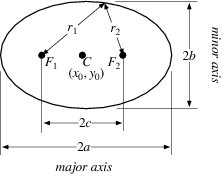
\includegraphics[height=1.5in]
    {Figures/EllipseGeometry.png}}
  \caption{\label{ref:EllipseGeometry} Caption}
\end{figure}

\begin{proof}
If the perimeter is maximized keeping $2c$ a constant, $(r_1 + r_2)$ is 
maximized \textit{because} $2c$ is a constant.  Maximizing $(r_1+r_2)$ 
maximizes a from the following relation with $2c$ being constant: $r_1 + 
r_2 = 2a$.  Combining the following relation, $b^2 = a^2 + c^2$, with the 
area of the ellipse, $A = \pi * a * b$, yields $A=\pi^{2}*a^{2}(a^{2} - 
c^2)$.  If $c$ is a constant and $a$ is maximized, then the maximal area 
is obtained from maximal $(r_1+r_2)$.  Which means the curve must be 
inside of the spheroid defined by the ellipse.  If the curve is not inside 
the spheroid then there is a point on the curve such that $(r_1+r_2)$ is 
larger and therefore the area is larger and therefore the volume is larger 
which means that $(r_1+r_2)$ was not maximized.
\end{proof}

Observe that there was no mention of the length of the curve inside of the 
spheroid, or the ruled area that the segment and curve could define.  
This is because there is no way this information can be known (without 
explicitly calculating the length of the curve/segment).  It is 
unfortunate that there is no way to quantify the discretization error of a 
curve except in terms of volume of the spheroids defined by each segment.  
This is non-intuitive, but no more specificity is possible.  The volumes 
would also be scale-dependent and offer no insight into how well the 
discretization approximates the curve -- without some context.


% Element Quality
\section{Element Quality}
A topic that has not been discussed thus far is element quality.  Element quality is an intuitive measure for surface elements, e.g. triangles; but how to define quality for a line segment?  In this context, the notion of quality refers to the change in length between two topologically adjacent segments.  For the purposes of representing the curve to a desired tolerance, grid quality is not a concern.  However, for most applications the grid quality directly affects downstream uses, e.g. CFD, CEM, etc…  Therefore some discussion of this topic is warranted.  Grid quality in terms of edge grids is most often defined in terms of growth ratio, i.e. the length of a segment divided by the length of a topologically adjacent segment.  If the growth ratio strongly deviates from unity then the sizes of neighboring elements are not similar.  This will lead to a large disparity in the size of surface elements generated from them and that “error” in the form of a large growth ratio will be present in both the surface grid and volume grid in the vicinity of that portion of the edge grid.  This kind of disparate length scales can cause problems for finite element methods, finite volume methods, etc…

        Traditionally edge grids are generated with an a priori defined growth ratio along with other parameters that ensure that the grid has good quality.  A priori quality measures can be included in the constraints used in the global optimization procedure in a similar fashion to how the minimum and maximum edge lengths were included.  Post hoc methods for quality control could include some type of smoothing or (other type of) optimization [find more methods].  The author acknowledges that set of constraints grows very quickly in number with respect to the number of grid points—albeit linearly.  There is the set that defines the topology (1), the set that defines the minimum(2) and maximum(3) edge lengths, and now two more for minimum(4) and maximum(5) growth rates—for a total of five times the number of points.  For the local procedure, minimum and maximum growth rates could be include by splitting an edge if the growth rate is too large or small.

        One final method is to use the output from the developed methods, the “optimal” grid, as input for a grid generator—which presumably has strict quality control measures in place.  This would be accomplished by using the point spacing values present at the end points of the discretization at the end points of the curve.  The resulting edge grid from the grid generator could then be analyzed for the purpose of determining how far it deviates from “optimality” in the interior of the curve.  For instance, given a node on a generated edge grid, $x_i$, the corresponding parameterized value of $u_i$ could be found.  A point spacing value could be calculated at $u_i$ and compared to an interpolated value on the “optimal” edge grid.  If the values are found to be too disparate, then a point spacing source could be added to adjust the point spacing at that location.  The point spacing source would control the spacing during grid generation so that the generated edge grid would more closely resemble the spacing values present in the “optimal” grid while maintaining the quality typically associated with grid generators. In practice this usually leads to generated grids that are more fine than required by precision bounds due to the quality constraints imposed during grid generation.



% Results
\section{Results}
Three curves were chosen to demonstrate the aspects of the developed methods. The first is a family of curves, $Lissajous$ curves (\Cref{fig:lissajous}), which are a combination of two perpendicular harmonic oscillations. This curve was chosen due to the sharp changes in curvature and self-intersecting nature. The second curve, a tricuspoid (\Cref{fig:tricuspoid}) was chosen for the sharp, discontinuous features. In \Cref{fig:lissajous,fig:tricuspoid,fig:lastfigure} the curve is shown in red and the discretization is shown in black with vertices highlighted by circles indicating their position. Each curve was scaled so that the parameterization, $t$, was normalized between zero and unity. In each case the curve was originally discretized using one segment corresponding to a vertex located at $t=0$ and $t=1$. Once the original discretization is created, the discretizations are refined using \Cref{alg:discreteoptimize}. Further results can be found in \Cref{tab:curvelength}. In this table, the true lengths of the curves can be found. The combined length of the segments in each discretization are also given with the actual arc-length deficit.

\begin{figure}[h!]
  \centering
  \begin{tabular}{ccc}
  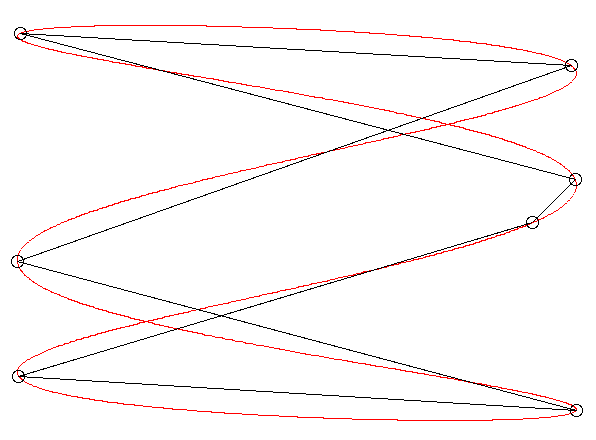
\includegraphics[width=0.3\linewidth]{Figures/lissajous01.png} &
  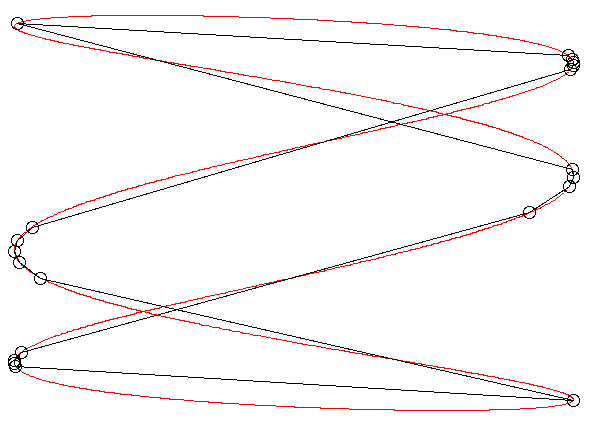
\includegraphics[width=0.3\linewidth]{Figures/lissajous001.png} &
  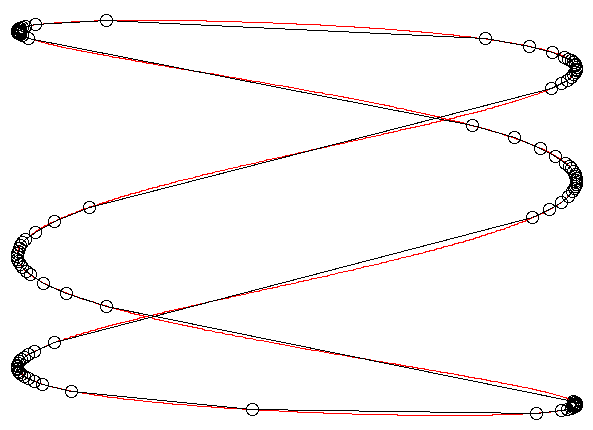
\includegraphics[width=0.3\linewidth]{Figures/lissajous0001.png}
  \end{tabular}
  \caption{\label{fig:lissajous} Lissajous Curves: 10\% deficit (left), 1\% deficit (middle), 0.1\% deficit (right)}
\end{figure}

For the Lissajous curve, the optimization can be seen to be effective and efficient with regards to only generating vertices where the curvature is high and not wasting vertices on the relatively ``straight'' portions of the curve. In addition, the self-intersection present on this curve did not impede the generation of an optimal edge-grid.

\begin{figure}[h!]
  \centering
  \begin{tabular}{ccc}
  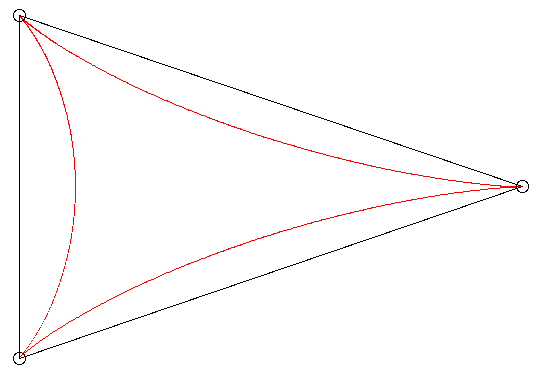
\includegraphics[width=0.3\linewidth]{Figures/tricuspoid01.png} &
  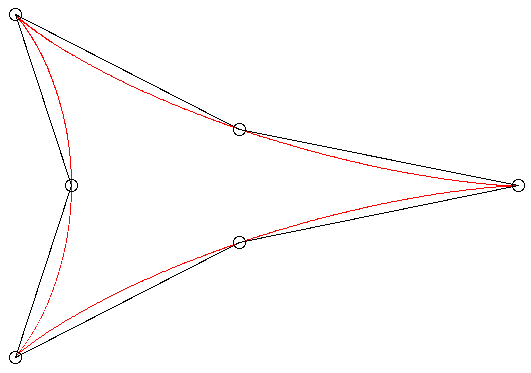
\includegraphics[width=0.3\linewidth]{Figures/tricuspoid001.png} &
  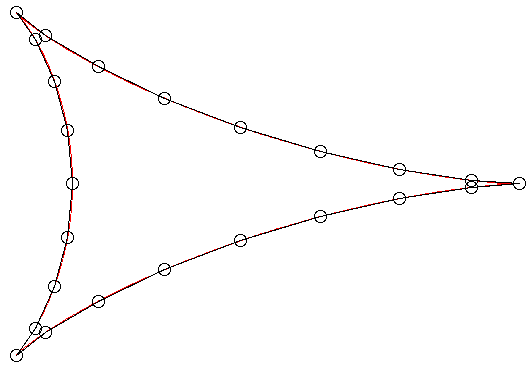
\includegraphics[width=0.3\linewidth]{Figures/tricuspoid0001.png}
  \end{tabular}
  \caption{\label{fig:tricuspoid} Tricuspoid Curve: 10\% deficit (left), 1\% deficit (middle), 0.1\% deficit (right)}
\end{figure}

For the Tricuspoid curve, the optimization can be seen to be accurate with regards to placing a vertex at the discontinuity. Placing a vertex at the discontinuity is efficient since not further nodes are required to capture that feature of the curve. It can be seen that further refinements are placed elsewhere on the curve.

\begin{figure}[h!]
  \centering
  \begin{tabular}{ccc}
  last & figure & here
  \end{tabular}
  \caption{\label{fig:lastfigure} Caption}
\end{figure}

\begin{table}[h!]
\caption{\label{tab:curvelength} Discretization length with respect to true curve length}
\begin{tabular}{cccc}
 & Lissajous Curve & Tricuspoid & last curve \\
True Length & 13.0653 & 16.0 & \\
10\% deficit criterion & 12.7123 (2.7\%) & 15.5885 (2.5\%) & \\
1\% deficit criterion & 12.8844 (1.3\%)& 15.8745 (0.78\%) & \\
0.1\% deficit criterion & 13.0436 (0.166\%) & 15.9906 (0.059\%) & 
\end{tabular}
\end{table}


% Conclusions
\section{Conclusions and Future Work}
%- Paragraph repeating abstract and confirming what was "promised".
% -reduce need for manual intervention - not many knobs and buttons
% -local optimization results in good representation wrt arc-length deficit
% -robustness, accuracy
%- adding {\it{a priori}} grid quality constraints to optimization problem \\
%- global optimization \\
%- surface optimization
An algorithm for edge grid discretization through local optimization was 
developed. In an effort to accelerate the process of grid generation, 
minimal user input is required for the developed method: a single 
parameter which is used as a limit for local refinement. The results show 
that the generated edge grid is optimal with respect to arc-length 
deficit. In addition, the process was shown to be robust to 
discontinuities, abrupt changes in curvature, and self-intersections. 
Results were shown here in two dimensions for ease of presentation. The 
developed algorithm is easily abstracted to three dimensional curves
through a the kernel for edge length calculation.

Future work would include a comparison to a global optimization problem 
formulated with the presented constraints and an additional constraint of 
a given number of edge grid points. Grid quality measures could also be 
included in the optimization problem via {\it a priori} quality 
constraints.

More work will also be done to abstract the problem from strictly 
one-dimensional simplices (edge grids) to two-dimensional simplices 
(triangles). While it was straightforward to determine which part of a 
curve an edge grid represents, it is non-trivial to determine which part 
of a surface a triangle represents. The development of a map between the 
planar elements representing a surface and the underlying geometry would 
be one of the chief tasks moving forward. Additionally, the edges, as well 
as the triangles, in the discretization must considered when optimizing 
the surface grid.

Finally, we will apply our edge and surface grid generation routines on 
problems stemming from real-world applications, including those from 
mechanical engineering and medicine.  One challenge that will need to be 
faced is the development of a surface grid generator which can develop 
an optimal representation of a surface from noisy data, e.g., medical
imaging. An engineering application would be to accelerate the mesh generation
process for fluids simulations by automatically generating surface meshes
that capture local geometry.


% Acknowledgments
\section{Acknowledgments}
The work of the second author is supported in part by NSF CAREER Award
ACI-1330056 (formerly OCI-1054459).


%
%
% BibTeX users please use
\bibliographystyle{plain}
\bibliography{References}
%
% Non-BibTeX users please follow the syntax
% the syntax of "referenc.tex" for your own citations
%%%%%%%%%%%%%%%%%%%%%%%%%%%%%%%%%%%%%%%%%%%%%%%%%%%%%%%%%%%%%%%%%%%%%%

%%%%%%%%%%%%%%%%%%%%%%%%%%%%%%%%%%%%%%%%%%%%%%%%%%%%%%%%%%%%%%%%%%%%%%

\printindex
\end{document}





